\subsection{$\phi^4$ Results}
\label{sec:phi4_results}

Any field theory is defined at the level of a Lagrangian.
For $\phi^4$ theory is given as
\begin{equation}
    \mathcal{L} = \frac12 \left(\partial_\mu \phi \right)^2 - \frac{m^2}{2}\phi^2 - g\phi^4.
\end{equation}

To obtain a Hamiltonian from a Lagrangian, a Legendre transformation is performed, in which an explicit set of coordinates must be chosen. 
The set of coordinates used in this paper, which lead to the simplest forms of the corresponding Hamiltonians, are front form (lightfront) coordinates \cite{Dirac1949}.
A discussion on lightfront coordinates will be given in appendix \ref{subsec:qft-hamiltonians}.

The $\phi^4$ Hamiltonian can be written as:
\begin{align}
    H = \sum_i &c_i a_i^\dagger a_i + \sum_{ijkl}c_{ijkl} \left(a_i^\dagger a_j^\dagger a_k^\dagger a_l + h.c. \right) + \nonumber\\
    &\sum_{ijkl}c_{ijkl}a_i^\dagger a_j^\dagger a_k a_l
\end{align}
where the values of the coefficients are omitted for brevity, but can be determined numerically.

Unlike the Quartic Harmonic Oscillator and the Static Massive Yukawa model, $\phi^4$ theory is defined based on a discretization of momentum modes.
In lightfront field theories, it is common to refer to the resolution of the model, which dictates the size of the momentum grid or the total number of momentum modes.
For those unfamiliar, the resolution can be thought of analogously to the molecular orbital basis in quantum chemistry simulations.
A further discussion on the physical meaning of resolution will be given in appendix \ref{subsec:qft-hamiltonians}.

\begin{figure*}
    \label{fig:phi4}
    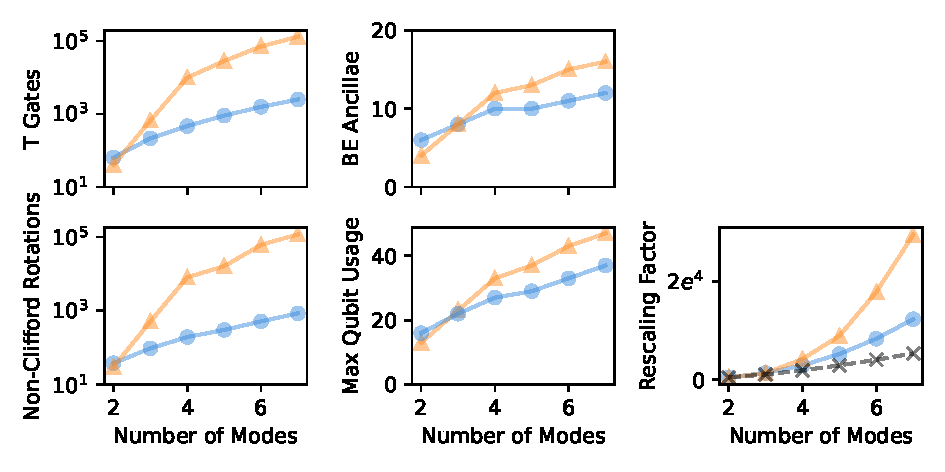
\includegraphics[width = 16cm]{figures/phi4-resolution-3.pdf}
    \caption{
        \textbf{$\phi^4$}
        The number of T gates (upper-left), number of non-Clifford rotations (lower-left), block-encoding ancillae (upper-middle), maximum number of qubits used (lower-middle), and rescaling factor (lower-right) are shown as a function of the number of momentum modes.
        The bosonic cutoff is fixed to $\Omega = 3$ and the parameters $g$ and $m_b$ are set to $1$ for all data points.
        Results for the ``Pauli - Expansion" method are shown as the orange triangles and results for LOBE are shown as the blue circles.
        The optimal rescaling factor, which is given by the L2 norm of the Hamiltonian, is shown as the dashed black crosses.
    }
\end{figure*}

Since the previous results establish that LOBE constructions are generally preferred when the bosonic cutoff is large, here we chose to look at the spacetime cost as a function of the total number of momentum modes.
In Figure \ref{fig:phi4}, we show the scaling of the spacetime costs associated with both the LOBE and Pauli Expansion block-encodings as a function of the number of modes.
For these estimates, the bosonic cutoff is fixed to $\Omega = 3$.
When the number of modes is small (low resolution), the LOBE and Pauli Expansion constructions require similar spacetime costs, with the Pauli Expansion block-encodings requiring \ws{one} fewer block-encoding ancilla when there are only two modes.
For higher resolutions (more modes), the LOBE constructions require signficantly fewer T gates and non-Clifford rotations, in addition to requiring fewer block-encoding ancillae, using fewer total qubits, and having smaller rescaling factors.
Notably, when $7$ momentum modes are used, the time cost for the LOBE construction is approximately two orders of magnitude smaller than the Pauli Expansion construction.
